\documentclass[conference]{IEEEtran}
\usepackage{fontspec}
\IfFontExistsTF{Times New Roman}{\setmainfont{Times New Roman}}{\setmainfont{TeX Gyre Termes}}
\usepackage{adjustbox,array,xurl,float}
\newcolumntype{L}[1]{>{\raggedright\arraybackslash}p{#1}}
\usepackage{graphicx,booktabs,amsmath,url,multirow,tikz}
\usetikzlibrary{arrows.meta,positioning,fit}
\usepackage[hidelinks]{hyperref}
\begin{document}

\title{Truy vấn văn bản--hình ảnh có khai thác đồ thị: so sánh CLIP, mạng nơ-ron đồ thị và AdaMF-MAT}

\author{\IEEEauthorblockN{25C11008 - Châu Ngọc Huy \quad 25C11020 - Hoàng Minh Thắng \quad 25C15014 - Nguyễn Đinh Quang Khánh\\
25C15004 - Võ Trần Đông Dương \quad 25C11075 - Phạm Thị Như Yến}
\IEEEauthorblockA{Học máy với dữ liệu đồ thị}}

\maketitle

\begin{abstract}
Nghiên cứu này đánh giá liệu scene graph và tri thức từ ConceptNet có cải thiện truy vấn văn bản--hình ảnh so với CLIP đóng băng hay không. Trên Visual Genome$\cap$MS-COCO và PSG$\cap$MS-COCO, các phương pháp dùng chung split, tập ứng viên top-100 và giao thức ba seed. GNN trên đồ thị nhãn--ảnh cải thiện MRR toàn tập test thêm 1,4--1,9 điểm phần trăm so với CLIP có adapter; khoảng tin cậy bootstrap 95\% không chứa 0. Xáo trộn cạnh làm kết quả thấp hơn baseline adapter, cho thấy cấu trúc cạnh có đóng góp. Mức cải thiện tập trung ở truy vấn trực tiếp; lợi ích trên truy vấn gián tiếp còn nhỏ. AdaMF-MAT được tái lập trong phạm vi một điểm trên MKG-W và MKG-Y, nhưng không vượt baseline khớp tên đối tượng khi áp dụng cho xếp hạng ảnh. Nghiên cứu chưa có kết quả định lượng về giải thích mô hình hoặc thực nghiệm trên MMKG tiếng Việt; các nội dung này được xem là giới hạn của phạm vi hiện tại.
\end{abstract}

\begin{IEEEkeywords}
truy vấn đa phương thức, CLIP, mạng nơ-ron đồ thị, đồ thị tri thức đa phương thức, khả năng giải thích
\end{IEEEkeywords}

\section{Giới thiệu}\label{sec:intro}
CLIP~\cite{clip} biểu diễn câu và ảnh trong cùng một không gian vectơ và xếp hạng ảnh theo độ tương đồng cosine. Cách làm này nhanh nhưng chỉ dựa trên độ giống nhau của biểu diễn: nó không dùng quan hệ có cấu trúc giữa đối tượng và khái niệm, và không cho biết vì sao một ảnh được trả về. Với truy vấn ``a child playing football'', nếu ảnh chỉ nhận ra được \emph{ball} và \emph{field}, một đường đi trong đồ thị tri thức có thể nối truy vấn với đúng ảnh.

Nghiên cứu tập trung vào vai trò của thông tin quan hệ trong truy vấn ảnh, thay vì huấn luyện lại một mô hình thị giác lớn. Chúng tôi so sánh CLIP đóng băng với các phương pháp xếp hạng lại dựa trên GNN và hoàn thiện MMKG bằng AdaMF-MAT. Đánh giá sử dụng một giao thức chung, kiểm soát rò rỉ dữ liệu và phân tích kết quả theo nhóm truy vấn trực tiếp/gián tiếp. Các thí nghiệm ablation trên hai bộ dữ liệu kiểm tra liệu cải thiện có đến từ nội dung cạnh hay chỉ từ năng lực tham số của mô hình.

\section{Công trình liên quan}\label{sec:rel}
\textbf{Truy vấn ảnh bằng ngôn ngữ.} CLIP~\cite{clip} học chung không gian ảnh--câu bằng đối sánh tương phản trên lượng lớn cặp ảnh--văn bản, và OpenCLIP~\cite{openclip} cung cấp bản huấn luyện lại trên dữ liệu mở. CLIP được giữ đóng băng trong toàn bộ báo cáo; mọi cải thiện đến từ phần xếp hạng lại.

\textbf{Scene graph cho truy vấn.} Johnson và cộng sự~\cite{sgret} dùng scene graph để truy vấn ảnh bằng quan hệ giữa đối tượng. Ở đây truy vấn là câu tự nhiên và đồ thị chỉ cung cấp tín hiệu phụ cho bộ xếp hạng lại đặt trên CLIP.

\textbf{GNN.} GCN~\cite{gcn}, GAT~\cite{gat} và GraphSAGE~\cite{sage} là ba cách lan truyền thông tin trên đồ thị: lấy trung bình có chuẩn hóa theo bậc, chú ý có trọng số học được, và gộp láng giềng được lấy mẫu. Cả ba được so sánh trong mục~\ref{sec:l1}.

\textbf{Đồ thị tri thức đa phương thức.} Các mô hình hoàn thiện MMKG như MKGformer~\cite{mkgformer}, NativE~\cite{native} và AdaMF-MAT~\cite{adamf} học biểu diễn thực thể từ cấu trúc, ảnh và văn bản. Khảo sát~\cite{survey} tổng hợp hướng nghiên cứu này. AdaMF-MAT được chọn vì có mã nguồn và dữ liệu công khai, cho phép tái lập và đánh giá trên giao thức truy vấn ảnh.

\textbf{Giải thích.} GNNExplainer~\cite{gnnexp} tìm đồ thị con và đặc trưng quan trọng cho dự đoán của một GNN. Vì giải thích cần phản ánh cơ chế xếp hạng, chúng tôi sử dụng đóng góp của cạnh vào điểm đồ thị làm giải thích và xem GNNExplainer như một tham chiếu.

\section{Dữ liệu và giao thức đánh giá}\label{sec:data}
\subsection{Dữ liệu}
\textbf{VG$\cap$COCO.} Ảnh Visual Genome (VG)~\cite{vg} có \texttt{coco\_id} (51\,208 ảnh) kết hợp 5 caption MS-COCO~\cite{coco} mỗi ảnh theo chia Karpathy. Truy vấn là caption; phía đồ thị là scene graph VG (đối tượng và quan hệ, tên đã chuẩn hóa). Chia: train 15\,000 ảnh (lấy mẫu, seed 0), val 2\,126, test 2\,138; 96\,381 caption. \textbf{PSG$\cap$COCO.} Bộ dữ liệu thứ hai, PSG~\cite{psg}, cùng cấu trúc (scene graph panoptic + caption Karpathy): 18\,186 ảnh (train 15\,000, val 1\,000, test 2\,186), 90\,974 caption, 133 nhãn ảnh và 674 khái niệm mở rộng từ ConceptNet~\cite{cn}.

\subsection{Tiền xử lý và trích đặc trưng VG}
Mã tiền xử lý \texttt{yen/prepare\_visual\_genome.py} nhận \texttt{scene\_graphs.json}, \texttt{image\_data.json} và \texttt{dataset\_coco.json} (Karpathy). Mã ghép ảnh VG với caption bằng \texttt{coco\_id}, xuất scene graph con vào \texttt{vg/objects.json} và \texttt{vg/relationships.json}, cùng \texttt{captions.json} và \texttt{splits.json} theo hợp đồng dữ liệu chung. Khi object thiếu khỏi danh sách nhưng quan hệ còn chứa tên endpoint, object được khôi phục từ tên đó; nếu chỉ còn ID thì quan hệ được ghi vào \texttt{preprocess\_report.json} và không tự gán nhãn suy đoán.

Mặc định, mã dùng split COCO-ID cố định \texttt{thang/kaggle\_results/split/split.json}: train 15\,000, val 2\,126 và test 2\,138 ảnh. Các ID này được ánh xạ sang VG-ID qua \texttt{image\_data.json}; mã kiểm tra split không giao nhau và dừng nếu thiếu ảnh, caption hoặc scene graph bắt buộc. Thay thế, \texttt{--random-split --seed 0 --ratios 0.8 0.1 0.1} tạo split xác định từ danh sách COCO-ID đã sắp xếp rồi xáo trộn; các VG-ID cùng COCO-ID luôn thuộc một tập. Kết quả và seed được lưu trong \texttt{splits.json} để các lần chạy dùng chung, không chia lại theo caption hay theo mô hình.

Mã \texttt{yen/extract\_visual\_genome\_features.py} dùng OpenCLIP đóng băng (mặc định ViT-B/32, \texttt{laion2b\_s34b\_b79k}) để mã hóa ảnh, caption và tên nhãn. Kết quả float32 đã chuẩn hóa L2 được lưu trong \texttt{features/image\_emb.npy}, \texttt{caption\_emb.npy}, \texttt{label\_emb.npy}, kèm các tệp ID, \texttt{labels.json} và \texttt{clip\_model.json}. Từ vựng dùng để tạo embedding nhãn chỉ lấy từ object của ảnh train; caption và ảnh val/test được mã hóa bằng encoder đóng băng, không dùng để cập nhật trọng số.

\subsection{Giao thức}
Hình~\ref{fig:pipe} tóm tắt pipeline. Mọi phương pháp dùng cùng tệp chia ảnh, cùng một mô hình CLIP (ViT-B/32, \texttt{laion2b\_s34b\_b79k}, đóng băng) và cùng bước chọn ứng viên: top-$K{=}100$ theo cosine; ảnh đúng nằm ngoài top-$K$ giữ nguyên hạng của CLIP. Điểm cuối là $s=\alpha\,z(\cos)+(1-\alpha)\,z(\text{đồ thị})$, trong đó $z(\cdot)$ là chuẩn hóa z-score theo truy vấn nhằm đưa hai thành phần về cùng thang đo; $\alpha$ \emph{chỉ} được chọn trên val. Số liệu báo cáo ở hai dạng: (a) gallery 1\,000 ảnh theo 3 seed (trung bình $\pm$ độ lệch chuẩn, kiểu COCO 1K); (b) toàn pool test (tất định) kèm kiểm định bootstrap ghép cặp theo truy vấn cho hiệu MRR giữa hai mô hình. Với mô hình học, seed điều khiển cả fold gallery và khởi tạo.

Tệp chia cố định (seed 0, Karpathy) và mã tạo chia nằm trong kho mã (Phụ lục B).

\subsection{Độ đo}
Với mỗi truy vấn có đúng một ảnh đúng (ảnh có caption đó), gọi $r$ là hạng của ảnh. Recall@$k=\mathbf{1}[r\le k]$ lấy trung bình trên truy vấn; hạng nghịch đảo trung bình $\mathrm{MRR}=\overline{1/r}$; $\mathrm{nDCG@}10=\overline{\mathbf{1}[r\le10]/\log_2(r+1)}$. Với bộ 24 truy vấn có nhiều ảnh dương, hạng được tính theo ảnh dương đứng đầu. Khoảng tin cậy 95\% (CI95) ở các bảng ghép cặp được tính bằng bootstrap lấy lại mẫu theo truy vấn, trên cùng thứ tự truy vấn của hai mô hình.

\textbf{Chống rò rỉ.} Split được tạo theo COCO-ID trước khi ánh xạ sang VG-ID, do đó các caption của cùng ảnh và các VG-ID trùng nguồn không thể rơi vào nhiều tập. Từ vựng nhãn dùng cho embedding lấy từ train; cạnh quan hệ scene graph và thống kê đồng xuất hiện chỉ tổng hợp từ ảnh train. Caption train là dữ liệu huấn luyện; val chỉ dùng chọn siêu tham số, early stopping và $\alpha$; test chỉ dùng báo cáo cuối. Đặc trưng CLIP có thể tính cho mọi split vì encoder đóng băng và không được fine-tune trên val/test. Trong cấu hình này, danh sách object của từng ảnh val/test vẫn được dùng làm đầu vào \texttt{contains} cho ảnh ứng viên; vì vậy kết quả giả định scene graph có sẵn tại suy luận. Nếu triển khai chỉ có ảnh thô, cần thay nhãn VG này bằng dự đoán của bộ phát hiện đối tượng và không được xem kết quả hiện tại là đánh giá end-to-end. Bộ 24 truy vấn quan hệ chỉ dùng để đánh giá.

\textbf{Nhóm truy vấn.} Giao thức tự gán: \emph{direct} nếu mọi khái niệm trong caption có mặt trong danh sách đối tượng của ảnh đúng, \emph{indirect} nếu có ít nhất một khái niệm không có mặt (cần suy ra qua từ đồng nghĩa hoặc quan hệ), còn lại là \emph{no\_concept}.



\subsection{Chi tiết cài đặt}
\begin{table}[t]
\caption{Thiết lập chính của từng thành phần.}\label{tab:impl}
\centering\footnotesize
\setlength{\tabcolsep}{3pt}
\begin{adjustbox}{max width=\columnwidth}
\begin{tabular}{lL{5.8cm}}
\toprule
Thành phần & Thiết lập\\\midrule
CLIP & ViT-B/32, \texttt{laion2b\_s34b\_b79k}, 512 chiều, chuẩn hóa L2, đóng băng\\
Ứng viên & top-100 theo cosine (FAISS \texttt{IndexFlatIP})\\
GNN & 2 tầng, ẩn 256, 4 đầu chú ý (GAT), batch 512, lr $10^{-3}$, $\tau=0{,}05$, dừng sớm theo MRR val (kiên nhẫn 4)\\
Huấn luyện GNN & InfoNCE trên caption train; đồ thị con theo batch (chính xác, có kiểm thử)\\
$\alpha$ & lưới bước 0,05, chọn trên val\\
AdaMF-MAT (tái lập) & chiều 200, batch 1024, 128 mẫu âm, lr $2\!\times\!10^{-5}$, 1000 epoch, lề 12 (MKG-W) / 4 (MKG-Y), seed 42\\
AdaMF-MAT (truy vấn ảnh) & chiều 200, lr $10^{-4}$, 104 epoch, 85,8 s/epoch, 1 seed\\
Phần cứng & GPU T4; một số lượt PSG và thử nghiệm chạy trên CPU cục bộ\\\bottomrule
\end{tabular}
\end{adjustbox}
\end{table}

\begin{figure*}[t]
\centering
\resizebox{\textwidth}{!}{%
\begin{tikzpicture}[>=Stealth, font=\small,
  box/.style={draw, rounded corners=2pt, align=center, minimum width=2.5cm, minimum height=1.15cm, inner sep=3pt, fill=white},
  src/.style={draw, rounded corners=2pt, align=center, minimum height=0.95cm, inner sep=3pt, fill=gray!12},
  grp/.style={draw, dashed, rounded corners=3pt, inner sep=5pt},
  arr/.style={->, thick}]
\node[box] (q) at (0,0) {Truy vấn\\(văn bản)};
\node[box] (c) at (3.2,0) {Mã hóa\\CLIP đóng băng};
\node[box] (k) at (6.6,0) {Top-$k$ ứng viên\\theo cosine (FAISS)};
\node[box, fill=green!12] (g) at (11.5,0) {Điểm đồ thị từng ứng viên\\(GNN, AdaMF-MAT)};
\node[box, minimum width=4.2cm] (r) at (15.8,0) {Xếp hạng lại\\$s=\alpha\,z(\cos)+(1-\alpha)\,z(g)$};
\node[box] (x) at (20.1,0) {Top-$k$ kết quả\\+ quan hệ/đường đi};
\node[box] (e) at (23.4,0) {Đánh giá\\Recall, MRR, fidelity};
\foreach \a/\b in {q/c,c/k,k/g,g/r,r/x,x/e} \draw[arr] (\a) -- (\b);
\node[src] (kg) at (11.5,-2.7) {Đồ thị: scene graph (VG, PSG),\\MMKG, ConceptNet\\(chỉ xây từ ảnh train)};
\node[src] (va) at (15.8,-2.7) {Tập validation:\\chọn $\alpha$ và siêu tham số};
\draw[arr] (kg.north) -- (g.south);
\draw[arr] (va.north) -- (r.south);
\node[grp, fit=(q)(k), label={[font=\small\bfseries]above:Truy hồi CLIP}] {};
\node[grp, fit=(g)(r)(kg)(va), label={[font=\small\bfseries]above:Xếp hạng đồ thị}] {};
\node[grp, fit=(x)(e), label={[font=\small\bfseries]above:Đánh giá}] {};
\end{tikzpicture}}
\caption{Quy trình đánh giá: CLIP tạo top-$k$ ứng viên, điểm đồ thị được kết hợp với cosine để xếp hạng lại, và kết quả được đánh giá bằng các độ đo truy hồi cùng phân tích giải thích.}\label{fig:pipe}
\end{figure*}

\section{Baseline truy hồi CLIP}\label{sec:l0}
Đặc trưng ảnh/caption mã hóa một lần bằng OpenCLIP, lập chỉ mục FAISS~\cite{faiss} (\texttt{IndexFlatIP}). Độ đo: Recall@1/5/10, MRR, nDCG@10. Bảng~\ref{tab:clip} cho kết quả text$\to$image; thiết lập chung ở Bảng~\ref{tab:impl}; image$\to$text (gallery 1K, test) đạt R@1 $74{,}10\pm0{,}96$ và MRR $81{,}82\pm0{,}84$.

\begin{table}[t]
\caption{CLIP thuần, text$\to$image, VG$\cap$COCO (\%).}\label{tab:clip}
\centering\footnotesize
\setlength{\tabcolsep}{3pt}
\begin{adjustbox}{max width=\columnwidth}
\begin{tabular}{lccccc}
\toprule
 & R@1 & R@5 & R@10 & MRR & nDCG\\\midrule
Test, 1K, 3 fold & $57{,}36\!\pm\!0{,}95$ & $84{,}08$ & $91{,}76$ & $69{,}23\!\pm\!0{,}68$ & $74{,}32$\\
Test, toàn pool & $48{,}31$ & $75{,}35$ & $84{,}08$ & $60{,}40$ & $65{,}51$\\
Val, 1K, 3 fold & $58{,}17\!\pm\!0{,}40$ & $84{,}74$ & $92{,}29$ & $69{,}92$ & $75{,}00$\\\bottomrule
\end{tabular}
\end{adjustbox}
\end{table}

Theo nhóm (test, 1K): direct R@1 $56{,}9$, indirect $57{,}5$, no\_concept $51{,}4$. Như vậy, theo cách gán nhóm tự động này, CLIP không yếu hơn rõ rệt ở nhóm gián tiếp; mục~\ref{sec:disc} quay lại điểm này.

\section{Xếp hạng lại bằng đồ thị và GNN}\label{sec:l1}
\subsection{Đồ thị}
Đỉnh gồm ảnh, nhãn đối tượng (2\,000 nhãn phổ biến nhất ở train) và khái niệm bổ sung. Cạnh gồm: \texttt{contains} (nhãn--ảnh, từ scene graph), \texttt{sg\_rel} (nhãn--nhãn, quan hệ trong scene graph, chỉ gộp từ ảnh train) và \texttt{concept} (ConceptNet: IsA, PartOf, UsedFor, AtLocation, CapableOf, HasA, Synonym; 16\,413 cạnh sau khi lọc theo từ vựng).

\subsection{Mô hình và điểm đồ thị}
Lần thử đầu dùng GAT nhận cả đặc trưng ảnh và cho MRR $+2{,}8$ so với CLIP, nhưng khi bỏ toàn bộ cạnh hoặc xáo cạnh, mức tăng không đổi. Mức tăng đó đến từ lớp chiếu (adapter) học được, vì GAT với self-loop trên ảnh chỉ là một MLP, không phải từ đồ thị. Do đó nền so sánh là CLIP kèm adapter không có cạnh, và mọi hiệu số trong báo cáo tính so với nền này.

Mô hình cuối (\emph{QA-Graph}): GNN (GCN/GAT/GraphSAGE, 2 tầng) chạy trên đồ thị \emph{nhãn} để cho vectơ $H_l$ mỗi nhãn $l$. Với truy vấn có tập khái niệm $\mathcal C$ (trích từ caption) và ảnh $i$ có tập nhãn $\mathcal L_i$, độ khớp của khái niệm $c$ với ảnh là $m(c,i)=\operatorname{softmax\text{-}max}_{l\in\mathcal L_i}\cos(u_c,H_l)$, và điểm đồ thị là trung bình $s_G=\frac1{|\mathcal C|}\sum_{c}m(c,i)$, cộng vào điểm adapter với một trọng số học được. Thiết kế này phụ thuộc truy vấn nên giữ được thông tin ``nhãn nào của ảnh khớp khái niệm nào của câu'' mà việc gộp mọi nhãn thành một vectơ ảnh làm mất. Bài kiểm tra cấu trúc trong mã: khi không có cạnh thì $s_G=0$ và thứ hạng trùng nền adapter. Huấn luyện bằng InfoNCE với caption train; $\alpha$ và siêu tham số chọn trên val.

\subsection{Kết quả chính}
Bảng~\ref{tab:main} và Hình~\ref{fig:main} tổng hợp 3 seed; $\Delta$MRR so với CLIP kèm adapter được tính ở seed~0 kèm CI95.

\begin{table}[t]
\caption{MRR (\%) toàn pool test, VG$\cap$COCO, mean$\,\pm\,$std 3 seed. $\Delta$ so với CLIP+adapter.}\label{tab:main}
\centering\small
\begin{adjustbox}{max width=\columnwidth}
\begin{tabular}{lcc}
\toprule
Cấu hình & MRR & $\Delta$ [CI95]\\\midrule
CLIP & 60,40 & --\\
CLIP + adapter (không cạnh) & $63{,}14\pm0{,}02$ & 0\\
+ đồ thị contains & $64{,}65\pm0{,}23$ & $+1{,}50$\\
+ contains + sg\_rel & $64{,}76\pm0{,}12$ & $+1{,}76$ [1,38; 2,16]\\
+ contains + ConceptNet (GAT) & $64{,}76\pm0{,}04$ & $+1{,}65$\\
+ contains + ConceptNet (GCN) & $64{,}56$ & --\\
+ contains + ConceptNet (SAGE) & $\mathbf{64{,}89\pm0{,}15}$ & $+1{,}93$ [1,49; 2,32]\\
+ đồ thị \emph{xáo cạnh} & $62{,}67\pm0{,}06$ & $-0{,}41$ [$-0{,}71$; $-0{,}11$]\\\bottomrule
\end{tabular}
\end{adjustbox}
\end{table}

\begin{figure}[t]
\centering
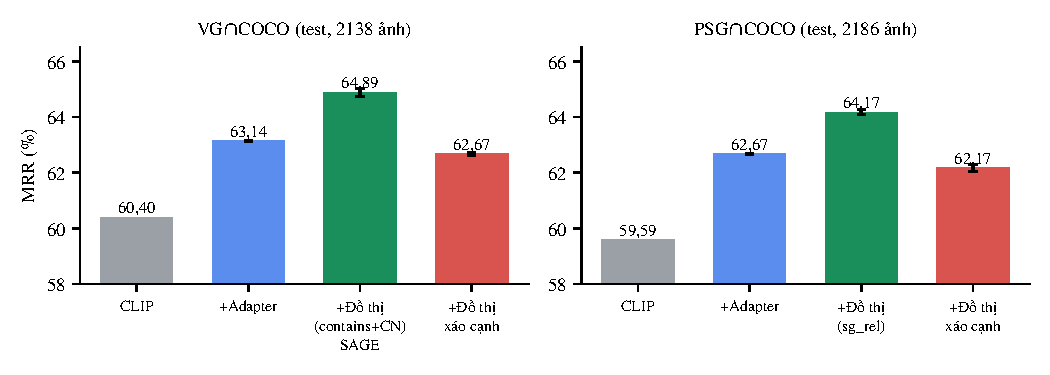
\includegraphics[width=\columnwidth]{figs/fig_main.pdf}
\caption{MRR toàn pool trên hai bộ dữ liệu. Thanh sai số là std 3 seed. Xáo cạnh tụt dưới nền adapter ở cả hai bộ.}\label{fig:main}
\end{figure}

Có bốn quan sát. (1) Đồ thị cải thiện $+1{,}4$ đến $+1{,}9$ MRR toàn pool so với adapter, CI95 không chứa 0 ở mọi biến thể, và $+4{,}3$ đến $+4{,}5$ so với CLIP. (2) Xáo cạnh làm điểm thấp hơn nền adapter ($-0{,}41$, có ý nghĩa): mô hình dùng nội dung của cạnh, nên lợi ích không do số tham số. (3) Chênh lệch giữa các GNN rất nhỏ: SAGE $\ge$ GAT $\ge$ GCN nhưng $\le0{,}3$ MRR, khoảng 1--2 std. (4) Có hay không \texttt{sg\_rel}, có hay không ConceptNet chênh $\le0{,}2$ MRR, nằm trong nhiễu; phần lớn lợi ích đến từ cạnh \texttt{contains} (đồ thị hai phía, một bước). Cấu hình được chọn cho các phân tích tiếp theo là \texttt{contains} + ConceptNet + SAGE, có MRR cao nhất trong các cấu hình được so sánh và không dùng cạnh \texttt{sg\_rel}.

\subsection{Bộ dữ liệu thứ hai}
Trên PSG (8 cấu hình $\times$ 3 seed), kết luận lặp lại: CLIP $59{,}59$; adapter $62{,}67\pm0{,}03$; QA-Graph $64{,}17\pm0{,}09$ ($+1{,}58$ [1,29; 1,89]); chỉ \texttt{contains} $64{,}35$; thêm ConceptNet $64{,}41$; xáo cạnh $62{,}12$ ($-0{,}50$ [$-0{,}78$; $-0{,}23$]). Ở PSG, 88\% truy vấn test là gián tiếp nhưng \texttt{sg\_rel} và ConceptNet vẫn không thêm đáng kể so với chỉ \texttt{contains}.

\section{Hoàn thiện MMKG bằng AdaMF-MAT}\label{sec:l2}
\subsection{Phương pháp}
AdaMF-MAT (LREC-COLING 2024) giải bài toán hoàn thiện đồ thị tri thức đa phương thức: dự đoán thực thể còn thiếu của bộ ba $(h,r,?)$ khi mỗi thực thể có thêm ảnh và văn bản. Quan sát của tác giả là các phương thức đóng góp không đều cho từng thực thể, nên mô hình hợp nhất có trọng số thích nghi giữa cấu trúc, ảnh và văn bản, và huấn luyện bằng cách tạo mẫu âm đối kháng (\emph{modality-adversarial training}) để cân bằng phương thức. Chúng tôi dùng nó như một bộ chấm điểm tính hợp lý của bộ ba (ảnh, \texttt{contains}, khái niệm).

\subsection{Tái lập trên MKG-W và MKG-Y}
Dùng mã và cấu hình của tác giả (chiều 200, batch 1024, 128 mẫu âm, 1000 epoch, seed 42) trên 2 GPU T4. Bảng~\ref{tab:repro} cho thấy mọi chênh lệch dưới 1 điểm so với bài báo; chỉ chạy 1 seed.

\begin{table}[t]
\caption{Tái lập AdaMF-MAT (lọc, trung bình hai chiều), \%.}\label{tab:repro}
\centering\small
\begin{adjustbox}{max width=\columnwidth}
\begin{tabular}{llcccc}
\toprule
Tập & & MRR & H@1 & H@3 & H@10\\\midrule
\multirow{2}{*}{MKG-W} & bài báo & 35,85 & 29,04 & 39,01 & 48,42\\
 & Tái lập & 35,68 & 28,98 & 38,68 & 48,13\\\midrule
\multirow{2}{*}{MKG-Y} & bài báo & 38,57 & 34,34 & 40,59 & 45,76\\
 & Tái lập & 39,10 & 34,59 & 41,23 & 46,68\\\bottomrule
\end{tabular}
\end{adjustbox}
\end{table}


Trên MKG-W, MRR khi dự đoán đuôi là $0{,}528$ nhưng khi dự đoán đầu chỉ $0{,}186$ (Hits@10: $0{,}677$ và $0{,}286$), trong khi MKG-Y gần đối xứng ($0{,}387$ và $0{,}395$). Thời gian huấn luyện đầy đủ là 3 giờ 32 phút (MKG-W, 12,7 s/epoch) và 2 giờ 14 phút (MKG-Y, 8,1 s/epoch).

\subsection{Tích hợp vào truy vấn ảnh}
Một MMKG được dựng từ cùng giao thức: 2\,000 khái niệm, 10\,264 ảnh, 31 quan hệ, 193\,962 bộ ba train (176\,736 \texttt{contains} và 17\,226 quan hệ khái niệm từ ảnh train). Điểm đồ thị của ảnh là tổng độ hợp lý của \texttt{contains} trên các khái niệm của caption; kết hợp theo công thức ở mục~II ($\alpha{=}0{,}75$ chọn trên val). Huấn luyện 104 epoch, 1 seed.

\subsection{Kết quả: trực tiếp và gián tiếp}
Bảng~\ref{tab:l2} (gallery 1K, 3 fold) cho thấy AdaMF-MAT cải thiện CLIP một chút ($+0{,}64$ MRR toàn pool, CI95 [0,33; 0,97]) nhưng chỉ ở nhóm direct. Ở nhóm indirect nó không hơn CLIP ($68{,}56$ so với $69{,}24$). Một baseline không dùng quan hệ (đếm khái niệm của câu có trong danh sách đối tượng của ảnh) bằng hoặc hơn AdaMF-MAT ở mọi chỉ số tổng ($+1{,}06$ MRR toàn pool).

\begin{table}[t]
\caption{MRR (\%) theo nhóm truy vấn, gallery 1K, 3 fold.}\label{tab:l2}
\centering\small
\begin{adjustbox}{max width=\columnwidth}
\begin{tabular}{lccc}
\toprule
Phương pháp & Tổng & direct & indirect\\\midrule
CLIP & $69{,}23\pm0{,}68$ & $69{,}33$ & $69{,}24$\\
CLIP + khớp tên (không quan hệ) & $70{,}21\pm0{,}84$ & $\mathbf{77{,}70}$ & $68{,}52$\\
CLIP + AdaMF-MAT & $69{,}77\pm0{,}74$ & $75{,}17$ & $68{,}56$\\\bottomrule
\end{tabular}
\end{adjustbox}
\end{table}


\subsection{Thêm adapter vào AdaMF-MAT}
Để so sánh với các mô hình GNN sử dụng adapter, chúng tôi bổ sung một adapter gồm hai phép tuyến tính $512\times512$ khởi tạo bằng đơn vị cho caption và ảnh, huấn luyện bằng InfoNCE ($\tau=0{,}05$, AdamW, lr $10^{-3}$) trên dữ liệu train, chọn epoch theo MRR val. Adapter này là phần mở rộng ngoài AdaMF-MAT, được chạy với một seed và chưa tinh chỉnh siêu tham số. Theo Bảng~\ref{tab:adapter}, phần lớn mức tăng đến từ adapter: đứng một mình nó đã $+2{,}01$ MRR toàn pool so với CLIP; AdaMF-MAT chỉ thêm $+0{,}59$ [0,31; 0,87] và chỉ ở nhóm direct ($71{,}47\to75{,}46$), còn nhóm indirect không cải thiện ($71{,}49\to71{,}21$). Baseline khớp tên trên nền adapter thêm $+1{,}05$ [0,80; 1,30], lớn hơn mức của AdaMF-MAT.

\begin{table}[t]
\caption{Có adapter, text$\to$image, test. MRR 1K là mean$\,\pm\,$std 3 fold (\%).}\label{tab:adapter}
\centering\footnotesize
\setlength{\tabcolsep}{3pt}
\begin{adjustbox}{max width=\columnwidth}
\begin{tabular}{lccc}
\toprule
Phương pháp & R@1 (1K) & MRR (1K) & MRR toàn pool\\\midrule
CLIP & $57{,}36\pm0{,}95$ & $69{,}23\pm0{,}68$ & 60,40\\
CLIP + AdaMF-MAT & $58{,}04\pm1{,}09$ & $69{,}77\pm0{,}74$ & 61,04\\
CLIP + adapter & $59{,}52\pm0{,}74$ & $71{,}47\pm0{,}55$ & 62,41\\
+ khớp tên & $60{,}98\pm0{,}83$ & $72{,}47\pm0{,}58$ & 63,46\\
+ AdaMF-MAT & $60{,}29\pm0{,}82$ & $71{,}99\pm0{,}58$ & 63,00\\\bottomrule
\end{tabular}
\end{adjustbox}
\end{table}

\subsection{Bộ 24 truy vấn trực tiếp/gián tiếp}
Từ \texttt{scene\_graphs.json} (108\,077 ảnh), nhóm sinh 24 truy vấn dạng ``chủ thể -- vị từ -- đối tượng'' (ví dụ ``hand feeding giraffe''): 12 trực tiếp, 12 gián tiếp. Chỉ dùng vị từ hành động; mỗi vị từ tối đa 3 truy vấn; hai thực thể đều xuất hiện $\ge200$ ảnh; loại các đối tượng mơ hồ. \emph{Trực tiếp}: ảnh dương là ảnh có bộ ba $s\!-\!p\!-\!o$ được chú thích (5--60 ảnh). \emph{Gián tiếp}: $s$ và $o$ nối với nhau chỉ qua một đối tượng thứ ba $x$ ($s\!\to\!x\!\to\!o$) và không có quan hệ $s$--$o$ nào trong chú thích. Các kiểm tra tự động đều đạt: không trùng truy vấn, không trùng cặp $(s,o)$, hai tập ảnh dương không giao nhau. Danh sách đầy đủ ở Phụ lục A. Hạn chế: chưa có ai xem ảnh, nên ảnh gián tiếp chỉ là ứng viên (đường đi hai bước không chứng minh ảnh thể hiện $s\,p\,o$); chú thích VG thưa nên có ảnh trực tiếp bị thiếu. Bộ này chỉ dùng để đánh giá, và các ảnh dương bị loại khỏi huấn luyện.

Trên thí nghiệm riêng này (gallery 1\,133 ảnh test, 1 seed, $\alpha$ chọn trên 51 truy vấn val), CLIP kèm AdaMF-MAT đạt MRR $0{,}677$ so với CLIP $0{,}630$, còn baseline chỉ đếm đối tượng đạt $0{,}881$. Lý do là ảnh dương và điểm đồ thị đều dựa trên cùng danh sách đối tượng được chú thích, nên sự có mặt của đối tượng gần như giải được bài toán. Với 12 truy vấn mỗi nhóm, một truy vấn là 8\% R@1, nên các chênh lệch 1--2 truy vấn không có ý nghĩa thống kê.

\subsection{So sánh ghép cặp với GNN}
Trên toàn pool test, seed~0, cùng thứ tự 10\,696 truy vấn, Bảng~\ref{tab:paired} cho $\Delta=$ (phương pháp) $-$ AdaMF-MAT; cấu hình GNN tốt nhất hơn AdaMF-MAT $+4{,}05$ MRR [3,62; 4,48], cả direct ($+4{,}70$) lẫn indirect ($+3{,}89$) (Hình~\ref{fig:group}). Xáo cạnh vẫn hơn AdaMF-MAT $+1{,}71$, do phần adapter. Khi ghép thêm adapter, AdaMF-MAT lên $63{,}00$ MRR toàn pool, vẫn dưới $65{,}09$ của GNN.


\begin{table}[t]
\caption{Kiểm định ghép cặp so với AdaMF-MAT, toàn pool test, seed 0, 10\,696 truy vấn. MRR (\%) và $\Delta$ [CI95 bootstrap] cho tổng.}\label{tab:paired}
\centering\footnotesize
\setlength{\tabcolsep}{3pt}
\begin{adjustbox}{max width=\columnwidth}
\begin{tabular}{lcc}
\toprule
Phương pháp & MRR & $\Delta$ so với AdaMF-MAT\\\midrule
CLIP + AdaMF-MAT & 61,04 & --\\
CLIP & 60,40 & $-0{,}64$ [$-0{,}97$; $-0{,}33$]\\
CLIP + khớp tên & 61,46 & $+0{,}42$ [0,16; 0,67]\\
CLIP + adapter (bỏ cạnh) & 63,16 & $+2{,}12$ [1,68; 2,54]\\
QA-Graph (contains+sg\_rel) & 64,92 & $+3{,}88$ [3,50; 4,26]\\
QA-Graph contains+CN (GAT) & 64,81 & $+3{,}77$ [3,36; 4,20]\\
QA-Graph contains+CN (SAGE) & 65,09 & $+4{,}05$ [3,62; 4,48]\\
QA-Graph xáo cạnh & 62,75 & $+1{,}71$ [1,30; 2,14]\\\bottomrule
\end{tabular}
\end{adjustbox}
\end{table}

\begin{figure}[t]
\centering
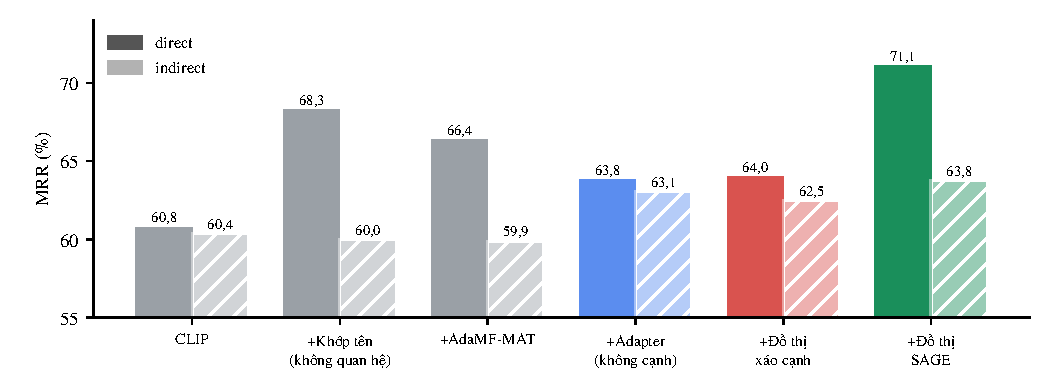
\includegraphics[width=\columnwidth]{figs/fig_group.pdf}
\caption{MRR toàn pool theo nhóm truy vấn (seed 0). Đồ thị thật tăng chủ yếu ở nhóm direct; xáo cạnh làm nhóm này thấp hơn nền adapter.}\label{fig:group}
\end{figure}

\section{Giải thích mô hình và phạm vi MMKG}\label{sec:xai}
\textbf{Phương pháp giải thích.} Giải thích phải đến từ chính cơ chế xếp hạng. Trong QA-Graph, điểm đồ thị của ảnh là tổng các đóng góp $m(c,i)$ theo khái niệm, mỗi $m(c,i)$ do nhãn khớp nhất và các cạnh GNN đã lan truyền đến nhãn đó. Vì vậy có thể trích cặp (nhãn khớp, đường đi cạnh trong đồ thị nhãn) làm giải thích. Mã trích xuất và can thiệp nằm ở \texttt{duong/xai} (\texttt{explain}, \texttt{perturbation}, \texttt{evaluate\_xai}). Để kiểm chứng, các cạnh được chọn bị xóa hoặc làm nhiễu rồi điểm đồ thị được tính lại; fidelity là độ giảm điểm và thay đổi hạng so với xóa ngẫu nhiên cùng số cạnh; sparsity là $1-\#\text{cạnh giải thích}/\#\text{cạnh ứng viên cục bộ}$; validity là việc cạnh tồn tại trong đồ thị và đúng lược đồ.

\textbf{Kết quả định lượng.} Chưa có kết quả fidelity, validity và sparsity trên các truy vấn thực với mô hình QA-Graph đã huấn luyện. Thử nghiệm trên dữ liệu tổng hợp chỉ kiểm tra đường chạy, không được xem là bằng chứng thực nghiệm và không được đưa vào so sánh định lượng.

\textbf{MMKG tiếng Việt.} Nghiên cứu hiện chưa xây dựng và đánh giá một MMKG tiếng Việt với nguồn dữ liệu, giấy phép và liên kết ảnh--thực thể được xác minh. Do đó, các kết luận thực nghiệm trong báo cáo chỉ giới hạn ở những bộ dữ liệu và giao thức được mô tả tại mục~\ref{sec:data}.

\section{Phân tích truy vấn thành công và thất bại}\label{sec:cases}
Từ kết quả CLIP trên test toàn pool, chúng tôi chọn 5 truy vấn thành công và 5 truy vấn thất bại (Bảng~\ref{tab:sf}). Đây là mẫu lỗi toàn cục, \emph{không} lấy cân bằng theo nhóm: cả 5 thành công mang nhãn \emph{indirect} của bộ gán nhãn tự động; trong 5 thất bại có 3 \emph{indirect}, 2 \emph{no\_concept}, và không có ví dụ \emph{direct}. Vì vậy không thể xem riêng 10 dòng này là so sánh đại diện direct--indirect. Theo định nghĩa tự động ở mục~\ref{sec:data}, \emph{indirect} chỉ có nghĩa là thiếu ít nhất một khái niệm trong object list; nó không chứng minh rằng truy vấn cần suy luận quan hệ.

Cả 5 truy vấn thành công có ảnh đúng ở hạng 1 (năm caption ứng với ba ảnh, vì ba caption cùng trỏ về một ảnh ``Pub''). Các câu về mèo/bàn/lông trang trí, súp/bông cải và biển ``PUB'' có nhiều tín hiệu thị giác cụ thể; nhãn ảnh vẫn có cat, desk, bowl, broccoli, bottle hoặc sign. Nhãn \emph{indirect} ở đây có thể do một phần mô tả hoặc cách diễn đạt không khớp chính xác với object vocabulary, chứ không nhất thiết cần cạnh quan hệ. Năm truy vấn thất bại có ảnh đúng ở hạng $1\,291$--$1\,784$ trên 2\,138 ảnh, thuộc ba kiểu:
\begin{itemize}
\item \emph{Caption không có nội dung thị giác}: ``There is no image here to provide a caption for'' và ``I am unable to see the image above'' (nhóm no\_concept): không phương pháp nào, kể cả đồ thị, cứu được vì không có khái niệm để nối.
\item \emph{Caption mơ hồ}: ``A photo of an outside with various things in the scene'' chỉ cho khái niệm ``outside'' không phân biệt ảnh nào.
\item \emph{Chú thích thưa}: ``a blue sign in front of leafy green trees'': danh sách đối tượng của ảnh đúng (hat, man, bench, tie, shirt, house) không chứa \emph{sign} hay \emph{tree}, nên khớp nhãn cũng không giúp.
\end{itemize}
Ở kiểu thứ hai và thứ ba, đồ thị chỉ giúp khi khái niệm truy vấn có thể nối đến nhãn ảnh; tuy nhiên, 10 ví dụ trên là kết quả CLIP, không phải dự đoán của QA-Graph. Để tách mức hiệu quả của hai nhóm, Bảng~\ref{tab:case-groups} báo cáo MRR nhóm từ kết quả chính thức trên gallery 1K, trung bình 3 seed. QA-Graph cải thiện nhiều hơn ở direct; mức tăng indirect chỉ $0{,}64$ điểm. Chưa có CI ghép cặp riêng cho từng nhóm nên không kết luận mức tăng indirect có ý nghĩa thống kê hay đã giải quyết suy luận quan hệ.

\begin{table}[t]
\caption{MRR (\%) theo nhóm tự động, test gallery 1K, trung bình $\pm$ std qua 3 seed.}\label{tab:case-groups}
\centering\footnotesize
\setlength{\tabcolsep}{3pt}
\begin{adjustbox}{max width=\columnwidth}
\begin{tabular}{lcc}
\toprule
Phương pháp & Direct & Indirect\\\midrule
CLIP + adapter (không cạnh) & $71{,}90\pm1{,}31$ & $71{,}80\pm0{,}39$\\
QA-Graph + ConceptNet (SAGE, không \texttt{sg\_rel}) & $78{,}71\pm1{,}12$ & $72{,}44\pm0{,}46$\\
Chênh lệch & $+6{,}81$ & $+0{,}64$\\\bottomrule
\end{tabular}
\end{adjustbox}
\end{table}

\textbf{Trường hợp cần suy luận quan hệ.} Cách phân nhóm tự động ở trên khác với benchmark quan hệ: direct yêu cầu bộ ba $(s,p,o)$ có trong annotation; indirect yêu cầu ảnh dương chỉ có đường nối hai bước $s\!\to\!x\!\to\!o$ và không có cạnh đích $(s,p,o)$. Ví dụ direct đối chứng trong \texttt{yen/relation\_queries.json} là ``A man is playing tennis'' (truy vấn d01, cạnh \texttt{man--playing--tennis}). Ví dụ indirect minh họa là $(\text{child},\text{plays},\text{football})$: chỉ thấy các thực thể riêng lẻ chưa đủ, mô hình phải dùng cấu trúc quan hệ đã học để phân biệt ảnh dương với ảnh âm có cùng thực thể nhưng thiếu cạnh cần thiết. Bộ sinh truy vấn trong \texttt{khanh/src/build\_eval\_queries.py} mô tả tiêu chí này; các truy vấn trong \texttt{yen/relation\_queries.json} hiện chưa được kiểm tra bằng mắt và chưa có kết quả xếp hạng đã căn chỉnh theo từng câu. Do đó hai truy vấn trên chỉ minh họa định nghĩa, không được tính là một trong 5 thành công hay 5 thất bại và không gán hạng dự đoán cho chúng.


\begin{table*}[t]
\caption{Năm truy vấn CLIP thành công (TC) và năm thất bại (TB), test toàn pool 2\,138 ảnh. Hạng là hạng ảnh đúng; nhãn direct/indirect/no\_concept theo quy tắc tự động, không đồng nghĩa với benchmark suy luận quan hệ.}\label{tab:sf}
\centering\footnotesize
\begin{tabular}{llcL{7.2cm}L{4.2cm}}
\toprule
 & Nhóm & Hạng & Caption & Đối tượng chú thích của ảnh đúng (rút gọn)\\\midrule
TC & indirect & 1 & Two cats on a desk and one wears pink feathers across the back. & paper, cat, bell, desk, boa, wall\\
TC & indirect & 1 & Two bowls of creamy soup and broccoli on a wood table. & spoon, table, bowl, napkin, broccoli, soup\\
TC & indirect & 1 & A sign with the word ``Pub'' hangs above several liquor bottles. & ice cube, bottle, letter, shelf, blender, sign\\
TC & indirect & 1 & a home bar with different drink ingredients under a large decorative sign saying ``PUB''. & (cùng ảnh với dòng trên)\\
TC & indirect & 1 & A sign with the word pub sits on a wall and underneath it on a table is a blender and three bottles\ldots & (cùng ảnh với dòng trên)\\\midrule
TB & no\_concept & 1\,784 & There is no image here to provide a caption for. & stone, wall, train car, mountain, locomotive\\
TB & indirect & 1\,694 & A photo of an outside with various things in the scene. & wing, engine, sky, plane, nose, tail\\
TB & indirect & 1\,361 & a blue sign in front of leafy green trees & hat, man, bench, tie, shirt, house\\
TB & indirect & 1\,319 & A full view of an outdoor space with many things to see. & foot, wire, dirt, elephant, fence, sky\\
TB & no\_concept & 1\,291 & I am unable to see the image above. & dot, table, glasses, keyboard, mug, cup\\\bottomrule
\end{tabular}
\end{table*}


\section{Thảo luận và hạn chế}\label{sec:disc}
\textbf{Vì sao đồ thị chưa giúp nhóm gián tiếp.} Phần tăng của QA-Graph nằm ở direct ($+6{,}4$ đến $+7{,}4$ MRR theo gallery) còn indirect chỉ $+0{,}3$ đến $+0{,}7$ (khoảng 1 std). Có ba cách giải thích, chưa được kiểm chứng riêng: (a) định nghĩa ``indirect'' của giao thức đo thiếu chú thích và từ đồng nghĩa nhiều hơn là suy luận quan hệ thật; (b) \texttt{sg\_rel} gộp từ đồng xuất hiện trên train rất dày (khoảng 50 láng giềng mỗi nhãn) nên làm nhòe danh tính nhãn, và khi chỉ giữ cạnh thưa (xuất hiện $\ge5$ lần) kết quả không khá hơn; (c) CLIP vốn đã mã hóa ``túi đối tượng'' tốt. ConceptNet là thứ duy nhất nhích nhóm indirect ($+0{,}5$ đến $+0{,}8$ ở seed~0) nhưng chênh vẫn trong nhiễu. Vì vậy chưa thể khẳng định đồ thị giúp truy vấn gián tiếp.


\textbf{Bài học phương pháp.} Với cả GNN và AdaMF-MAT, nền so sánh quyết định kết luận: so với CLIP thô, hầu hết mô hình có học đều tốt hơn, nhưng phần lớn mức tăng đến từ lớp chiếu học được. Một baseline không dùng quan hệ (khớp tên đối tượng) là phép thử rẻ: nếu phương pháp dùng quan hệ không vượt nó thì chưa có bằng chứng quan hệ đóng góp. Ablation xáo cạnh thuyết phục hơn ablation bỏ cạnh vì giữ nguyên số tham số và mật độ đồ thị.

\textbf{Các yếu tố ảnh hưởng đến tính hợp lệ.} (i) Nhóm direct/indirect do giao thức gán dựa trên chính danh sách nhãn mà đồ thị dùng, nên có nguy cơ vòng lặp: khái niệm có mặt trong nhãn thì được xếp ``direct'' và đồ thị dễ khớp. (ii) Chú thích scene graph thưa, nên nhãn thiếu có thể bị tính là lỗi của mô hình. (iii) Caption COCO chỉ có một ảnh đúng, trong khi nhiều ảnh khác cũng mô tả đúng; các độ đo thứ hạng vì thế bị đánh giá thấp một cách hệ thống và giống nhau cho mọi phương pháp. (iv) Ba seed của giao thức chủ yếu là ba fold gallery, và với CLIP đóng băng độ lệch chuẩn rất nhỏ (ví dụ $\pm0{,}02$ cho adapter), nên không phản ánh đầy đủ bất định của việc huấn luyện.

\textbf{Hạn chế.} (1) AdaMF-MAT chỉ huấn luyện một seed (ba seed của giao thức là ba fold gallery); chất lượng suy luận quan hệ trên đồ thị COCO yếu (MRR $0{,}072$, Hits@1 $\approx0$ khi kiểm tra các quan hệ khái niệm giữ lại) trong cấu hình 104 epoch, so với 1000 epoch khi tái lập; chưa xác định nguyên nhân. (2) Bộ 24 truy vấn chưa được kiểm tra bằng mắt và chưa đánh giá theo giao thức chung. (3) Thí nghiệm ẩn đối tượng (để presence-only thất bại và chỉ quan hệ mới suy ra được) đã chuẩn bị nhưng chưa chạy. (4) Giải thích định lượng và MMKG tiếng Việt chưa có số liệu (mục~\ref{sec:xai}). (5) Chưa chạy đồ thị ngẫu nhiên thay thế, chưa vẽ độ nhạy theo $\alpha$ và chưa dùng Wikidata hay NativE. (6) AdaMF-MAT trên pipeline chung mới được đánh giá trên VG$\cap$COCO.

\section{Kết luận}
Đồ thị cải thiện truy vấn ảnh một cách đo được và được ablation xác nhận: $+1{,}4$ đến $+1{,}9$ MRR so với nền có adapter trên hai bộ dữ liệu, và xáo cạnh làm điểm thấp hơn nền. Lợi ích tập trung ở truy vấn trực tiếp. AdaMF-MAT tái lập đúng bài báo nhưng không vượt baseline khớp tên khi dùng cho truy vấn ảnh. Các bước tiếp theo là kiểm tra truy vấn gián tiếp bằng cách ẩn đối tượng, thêm tri thức từ Wikidata và hoàn thành giải thích định lượng.

\section{Tái lập và khai báo}
Mã nguồn, lệnh chạy và hướng dẫn tái lập được lưu tại \url{https://github.com/Chau-Ngoc-Huy/graphml-project3}; giao diện kết quả CLIP tại \url{https://minhthang03.github.io/mmxai-task1-clip-baseline/web/}. Nhật ký thí nghiệm được lưu trong kho mã; hiện chưa có liên kết Weights \& Biases công khai. Nghiên cứu sử dụng mã nguồn mở của AdaMF-MAT và OpenCLIP, cùng các bộ dữ liệu có giấy phép công khai được nêu tại mục~\ref{sec:data}. Công cụ AI được sử dụng để hỗ trợ viết mã và biên tập bản thảo; các tác giả chịu trách nhiệm về nội dung và số liệu được báo cáo.


\section*{Phụ lục A: Các truy vấn đánh giá trực tiếp và gián tiếp}
\begin{table}[H]
\centering\footnotesize
\setlength{\tabcolsep}{3pt}
\begin{adjustbox}{max width=\columnwidth}
\begin{tabular}{L{3.9cm}L{3.9cm}}
\toprule
Trực tiếp (số ảnh dương) & Gián tiếp (số ảnh dương)\\\midrule
zebra standing on field (6) & woman holding boy (28)\\
boy eating food (10) & person sitting on horse (19)\\
hand feeding giraffe (10) & truck pulling trailer (10)\\
people standing on street (15) & person holding leash (17)\\
woman walking on sand (8) & man pulling luggage (10)\\
cow eating hay (13) & person playing with snowboard (10)\\
person driving bus (14) & person carrying luggage (5)\\
elephant carrying man (9) & person holding donut (5)\\
people watching person (7) & horse carrying person (7)\\
people riding bus (8) & man standing on floor (56)\\
people walking on walkway (6) & cat sitting on bed (26)\\
boy watching tv (5) & broccoli sitting on plate (38)\\\bottomrule
\end{tabular}
\end{adjustbox}
\end{table}

\section*{Phụ lục B: Tái lập thí nghiệm}
Môi trường gồm Python 3, PyTorch, \texttt{open\_clip}, PyTorch Geometric và FAISS; các thí nghiệm chính chạy trên GPU T4, một số lượt chạy cục bộ dùng CPU. Để tạo bundle Visual Genome theo hợp đồng MMXAI, chạy:
\begin{verbatim}
python yen/prepare_visual_genome.py --scene-graphs <scene_graphs.json> --image-data <image_data.json> --coco-captions <dataset_coco.json>
python yen/extract_visual_genome_features.py --data yen/data/visual_genome_mmxai --images-dir <VG_100K> <VG_100K_2>
\end{verbatim}
Lệnh đầu mặc định dùng split COCO-ID cố định; dùng \texttt{--random-split --seed 0 --ratios 0.8 0.1 0.1} để tạo split riêng. Đặc tả đầu vào, đầu ra và biện pháp chống rò rỉ ở mục~\ref{sec:data}; dữ liệu gốc và embedding không được đưa vào Git. Notebook \texttt{thang/task1\_clip\_baseline\_kaggle.ipynb} tái tạo benchmark, split và \texttt{task1\_bundle}. Pipeline GNN nằm trong \texttt{huy/} (lệnh \texttt{make local}/\texttt{make push}, cấu hình trong \texttt{src/mmxai/experiments}); các notebook AdaMF-MAT là \texttt{khanh/kaggle/protocol\_adamf\_kaggle.ipynb} (khoảng 3 giờ trên T4$\times$2) và \texttt{khanh/kaggle/adamf\_mat\_kaggle.ipynb}; so sánh ghép cặp được thực hiện bằng \texttt{khanh/tools/paired\_vs\_huy.py}. Chi tiết phụ thuộc từng thành phần được mô tả trong README tương ứng.

\begin{thebibliography}{99}
\bibitem{clip} A. Radford \emph{et al.}, ``Learning transferable visual models from natural language supervision,'' in \emph{Proc. Int. Conf. Mach. Learn. (ICML)}, 2021.
\bibitem{openclip} G. Ilharco \emph{et al.}, ``OpenCLIP.'' [Online]. Available: \url{https://github.com/mlfoundations/open_clip}
\bibitem{sgret} J. Johnson \emph{et al.}, ``Image retrieval using scene graphs,'' in \emph{Proc. IEEE Conf. Comput. Vis. Pattern Recognit. (CVPR)}, 2015.
\bibitem{gcn} T. N. Kipf and M. Welling, ``Semi-supervised classification with graph convolutional networks,'' in \emph{Proc. Int. Conf. Learn. Represent. (ICLR)}, 2017.
\bibitem{gat} P. Veli\v{c}kovi\'{c} \emph{et al.}, ``Graph attention networks,'' in \emph{Proc. Int. Conf. Learn. Represent. (ICLR)}, 2018.
\bibitem{sage} W. L. Hamilton, R. Ying, and J. Leskovec, ``Inductive representation learning on large graphs,'' in \emph{Adv. Neural Inf. Process. Syst. (NeurIPS)}, 2017.
\bibitem{mkgformer} X. Chen \emph{et al.}, ``Hybrid transformer with multi-level fusion for multimodal knowledge graph completion,'' in \emph{Proc. Int. ACM SIGIR Conf. Res. Dev. Inf. Retr.}, 2022.
\bibitem{native} Y. Zhang \emph{et al.}, ``NativE: Multi-modal knowledge graph completion in the wild,'' in \emph{Proc. Int. ACM SIGIR Conf. Res. Dev. Inf. Retr.}, 2024.
\bibitem{adamf} Y. Zhang \emph{et al.}, ``Unleashing the power of imbalanced modality information for multi-modal knowledge graph completion,'' in \emph{Proc. Joint Int. Conf. Comput. Linguist., Lang. Resour. Eval. (LREC-COLING)}, 2024, arXiv:2402.15444.
\bibitem{survey} Z. Zhu \emph{et al.}, ``Knowledge graphs meet multi-modal learning: A comprehensive survey,'' arXiv:2402.05391, 2024.
\bibitem{gnnexp} R. Ying \emph{et al.}, ``GNNExplainer: Generating explanations for graph neural networks,'' in \emph{Adv. Neural Inf. Process. Syst. (NeurIPS)}, 2019.
\bibitem{vg} R. Krishna \emph{et al.}, ``Visual Genome: Connecting language and vision using crowdsourced dense image annotations,'' \emph{Int. J. Comput. Vis.}, vol. 123, no. 1, pp. 32--73, 2017.
\bibitem{coco} X. Chen \emph{et al.}, ``Microsoft COCO captions: Data collection and evaluation server,'' arXiv:1504.00325, 2015; A. Karpathy and L. Fei-Fei, ``Deep visual-semantic alignments for generating image descriptions,'' in \emph{Proc. IEEE Conf. Comput. Vis. Pattern Recognit. (CVPR)}, 2015.
\bibitem{psg} J. Yang \emph{et al.}, ``Panoptic scene graph generation,'' in \emph{Proc. Eur. Conf. Comput. Vis. (ECCV)}, 2022.
\bibitem{cn} R. Speer, J. Chin, and C. Havasi, ``ConceptNet 5.5: An open multilingual graph of general knowledge,'' in \emph{Proc. AAAI Conf. Artif. Intell.}, 2017.
\bibitem{faiss} J. Johnson, M. Douze, and H. J\'{e}gou, ``Billion-scale similarity search with GPUs,'' \emph{IEEE Trans. Big Data}, vol. 7, no. 3, pp. 535--547, 2021.
\end{thebibliography}
\end{document}
